 																							                               	%---Cyrcé---%
%%%%%%%%%%%%%%%%%%%%%%%%%%%%%%%%%%%%%%%%%%%%%%%%%%%%%%%%%%%%%%%%%%%%%%%%%%%%%%%%%%%%%%%%%%%%%%%%%%

\documentclass[a4paper,11pt]{article}

%---Packages utilisés
\usepackage[utf8]{inputenc}
\usepackage[T1]{fontenc}
\usepackage[frenchb]{babel}
\usepackage{indentfirst}
\usepackage[]{graphicx}
\usepackage{amsmath}
\usepackage{ccaption}
\usepackage{vmargin}
\usepackage{textcomp}
\usepackage{fancyhdr}
%\usepackage[avantgarde]{quotchap}
\usepackage[Lenny]{fncychap}
\usepackage{cite}

\fancypagestyle{plain}{
\fancyhead[]{}
\fancyfoot[R]{\thepage}
\renewcommand{\headrulewidth}{0pt}}

%---Nouvelles commandes
\newcommand{\cyrce}{\textsc{Cyrcé}}
\newcommand{\Root}{\textsc{Root}}
\renewcommand{\baselinestretch}{1.2}
\newcommand{\alp}{$\alpha$}
\newcommand{\Asta}{$^{211}$At}
\newcommand{\AstaIso}{$^{210}$At}

%\renewcommand{\chaptermark}[1]{%
% \markboth{\thechapter . \ #1}{}}

%---Mise en page
\setlength{\parindent}{2ex}
%\pagestyle{fancy}

%---Début du document
\begin{document}

%---Marges du document
\setmarginsrb{3.5cm}{1.5cm}{1.5cm}{2cm}{2ex}{3ex}{2ex}{5ex}
%1 est la marge gauche
%2 est la marge en haut
%3 est la marge droite 
%4 est la marge en bas
%5 fixe la hauteur de l'etête
%6 fixe la distance entre l'entte et le texte
%7 fixe la hauteur du pied de page
%8 fixe la distance entre le texte et le pied de page
%
%\chapterstyle{veelo}
%\renewcommand{\sectionmark}[1]{\markright{\thesection\ #1}}
\lhead[]{}
\fancyfoot[C]{}
\fancyfoot[R]{\thepage}

%%%%%%%%%%%%%%%%
\begin{center}
\subsection*{Analyse des données issues des irradiations sur \cyrce\ (Avril 2017)}
\end{center}

\subsection*{Rappel de l'ensemble des irradiations}
\begin{center}
\begin{tabular}{lrrrrcl}
Fichier&pA&pos.&MeV&Gy&bdf/signal/bdf&Notes\\
\hline
\hline
C\_1000\_position\_00\_1&1.0&0&23.87&&30/30/30&\\
C\_1000\_position\_00\_2&1.0&0&23.87&&30/30/30&\\
C\_1000\_position\_00\_3&1.0&0&23.87&&30/30/30&\\
C\_1000\_position\_05\_1&1.0&5&20.42&&60/30/30&\\
C\_1000\_position\_10\_1&1.0&10&16.32&&30/30/30&\\
C\_1000\_position\_15\_1&1.0&15&11.13&&30/30/30&\\
C\_1000\_position\_17\_1&1.0&17&8.47&&30/30/30&\\
C\_500\_position\_00\_1&0.5&0&23.87&&30/30/30&\\
C\_2000\_position\_00\_1&2.0&0&23.87&&30/30/30&\\
C\_1000\_position\_pt\_1&1.0&pt&&1&&décimation 1/100\\
C\_1000\_position\_pt\_2&1.0&pt&&10&&décimation 1/100\\
C\_10000\_position\_pt\_1&10.0&pt&&10&&sans PM\\
C\_10000\_position\_pt\_2&0.0&pt&&0&&bruit de fond\\
C\_10000\_position\_pt\_3&10.0&pt&&10&&sans PM\\
\hline
\end{tabular}
\end{center}

\subsection*{Soustraction du bruit de fond}
La forme particulière du bruit de fond nécessite un traitement un peu plus poussé qu’une simple soustraction de sa valeur moyenne prise sur les périodes pré et post signal.
C'est d'autant plus essentiel que le bruit de fond peut être par moment supérieur au signal.
\begin{figure}[h]
\begin{center}
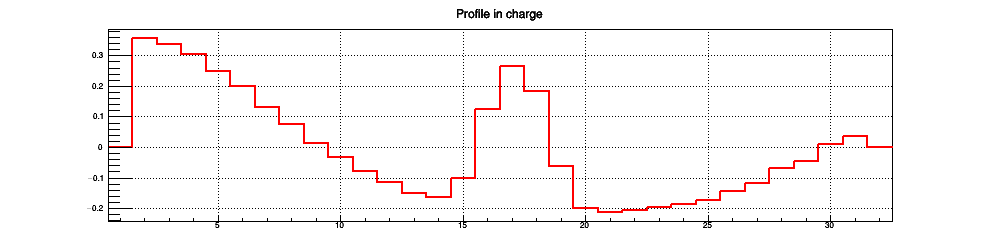
\includegraphics[scale=0.4]{SFB_396p.png} 
\caption{\label{fig:396p}\footnotesize{Profil X en charge obtenu sur une intégration de 2.4 ms en milieu d'irradiation}}
\end{center}
\end{figure}

\begin{figure}[h]
\begin{center}
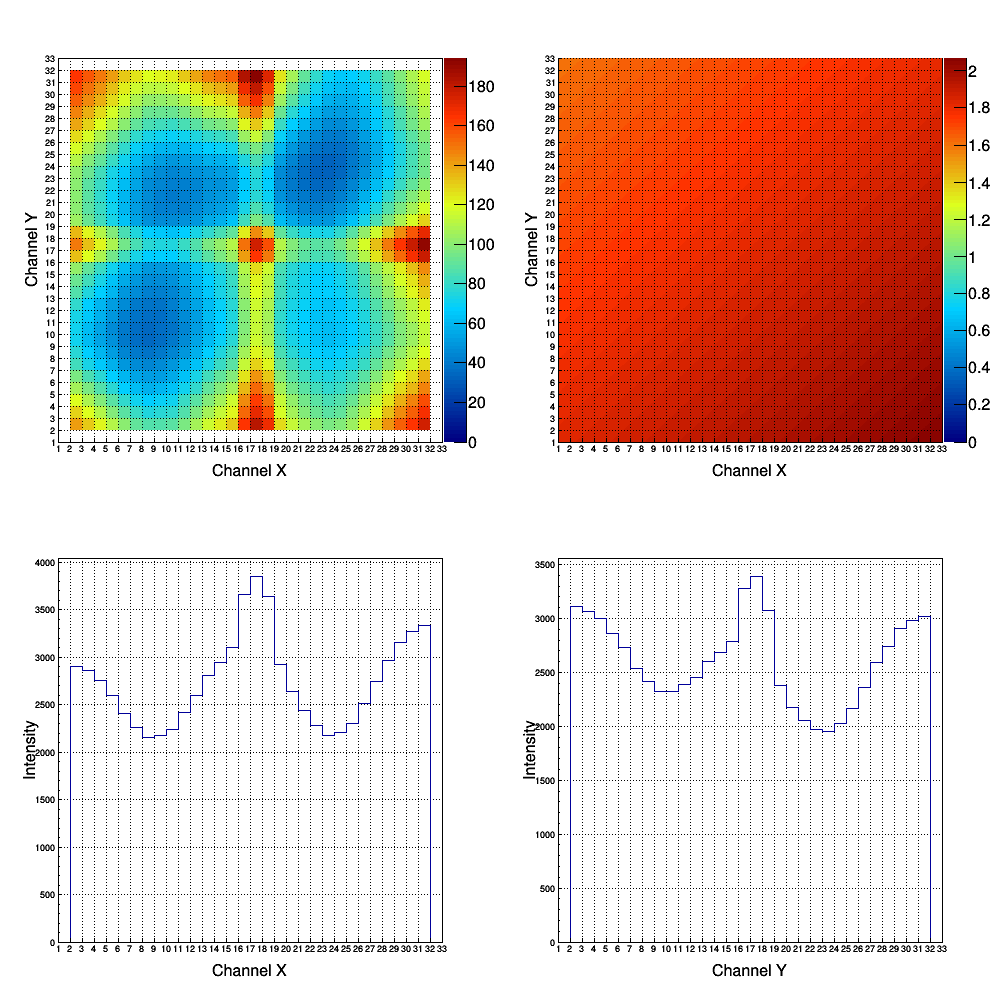
\includegraphics[scale=0.4]{Imagep.png} 
\caption{\label{fig:imagep}\footnotesize{Cartes du signal (haut à gauche) et de reconstruction (haut à droite) de l'irradiation et profils en X et Y}}
\end{center}
\end{figure}

Cela amène notamment aux résultats d'analyse inexploitables obtenus en sortie de \cyrce\ que j'avais pu vous montrer là-bas.
Le programme d'analyse qui s'attend à ne trouver qu'un seul pic se perd totalement et est incapable d'ajuster la gaussienne de reconstruction. 
Nous retrouvons bien les formes sinusoïdales du bruit de fond sur les deux profils.
En étudiant plus finement ce bruit de fond, nous n'avons pu trouver son origine. 
Les hypothèses que nous avions envisagées, comme la ventilation ou les pompes à vide, ayant des fréquences proches du Hz, nous aurions dû retrouver leurs traces dans la représentation temporelle des cartes du signal.

Or, si nous pouvons nettement observer une forme sinusoïdale sur chaque trame, celles-ci sont totalement différentes, voire en opposition de phase, d'une trame à la suivante. 
La fréquence d'acquisition étant de 2.4 ms, cela implique qu'elle doit être du même ordre de grandeur pour l'origine du bruit. 
Ceci nous oblige donc à traiter la soustraction de ce bruit de fond trame par trame, indépendamment les unes des autres.

Un des avantages du faisceau de \cyrce\ est d'être parfaitement stable en position et centré. 
Nous savons donc par avance où il va taper et combien de pistes seront touchées. 
Nous pouvons en excluant ces dernières effectuer un ajustement sur les pistes restantes et ainsi évaluer le bruit de fond sur celles recevant un signal. 
Je suis parti sur un simple ajustement polynomial de degré 8 (le maximum offert par \Root\ est de 9 mais la convergence ne se faisait plus) histoire de tester la faisabilité d'une telle analyse et de vérifier que le processus ne serait pas trop chronophage. 
Pour un fichier de 10 minutes d'acquisition, le temps nécessaire d'analyse est de l'ordre de 2 minutes 30, contre 20 secondes sans cette méthode. 
Cela laisse supposer qu'un tel calcul devrait être possible en temps réel.
\begin{figure}[h]
\begin{center}
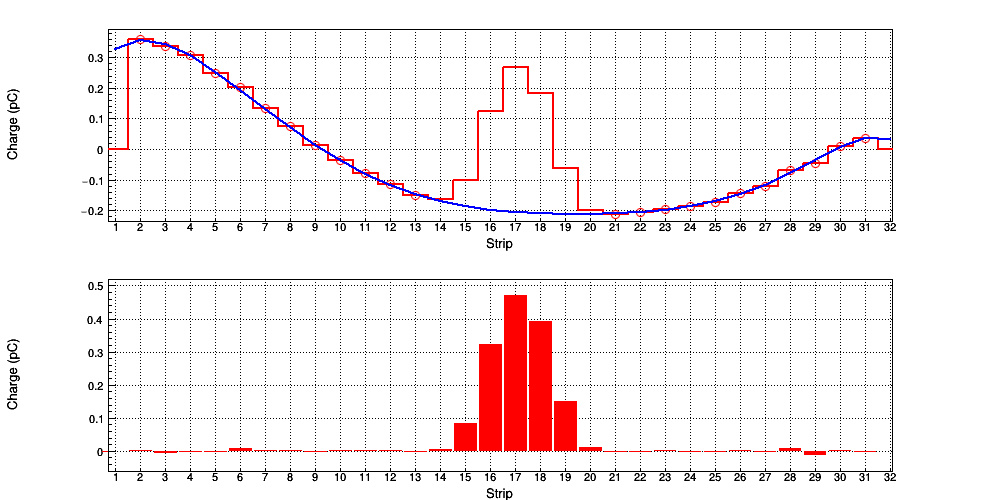
\includegraphics[scale=0.4]{SFB_396.png} 
\caption{\label{fig:396}\footnotesize{Les pistes non-exclues sont représentées avec le rond rouge, la courbe bleue montre l'ajustement réalisé et le graphique en bas le signal finalement obtenu après soustraction de ce bruit de fond}}
\end{center}
\end{figure}

Une telle méthode semble nous amener à des résultats cohérents et exploitables.
Nous retrouvons une zone centrale où se dégage parfaitement le pic, des zones extérieures nulles et le programme peut ainsi reconstruire une carte d'irradiation 2D, figure \ref{fig:imagep}.
\begin{figure}[h]
\begin{center}
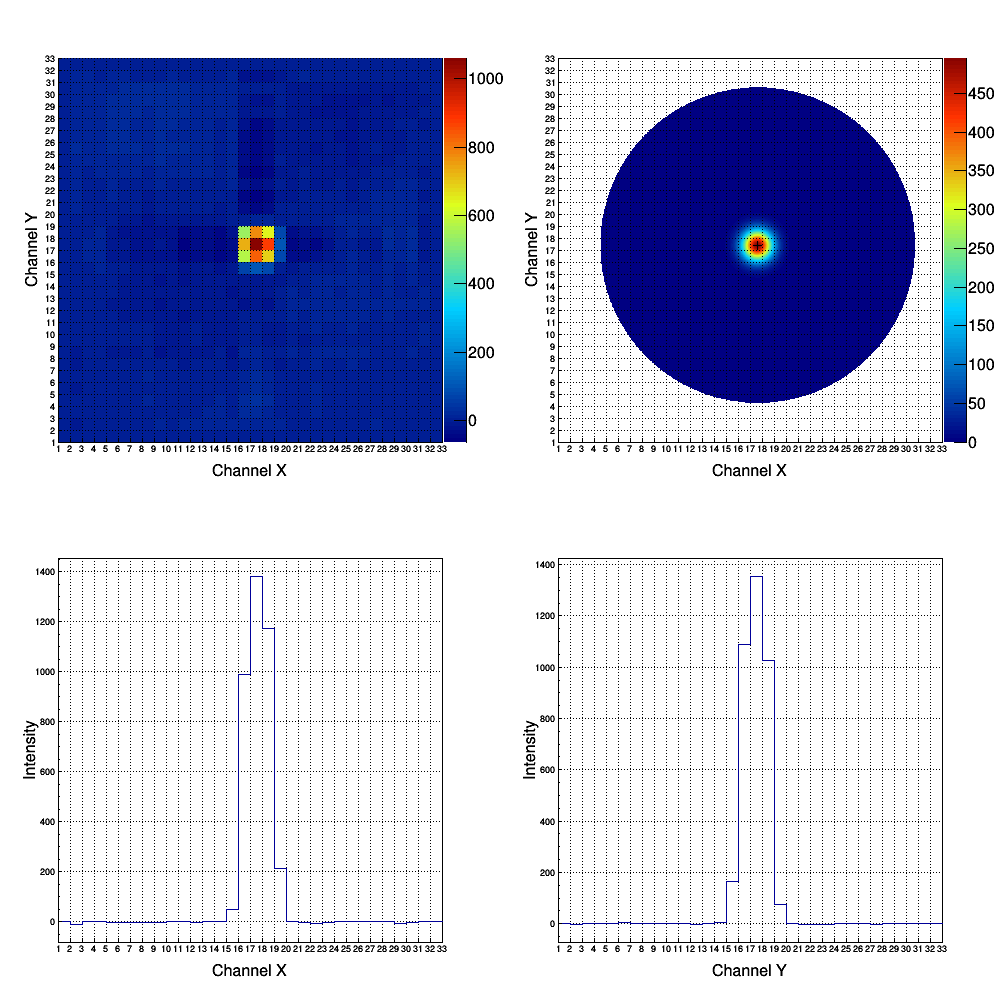
\includegraphics[scale=0.4]{Image.png} 
\caption{\label{fig:image}\footnotesize{Résultats de l'analyse obtenus avec la nouvelle méthode pour le même fichier que pour la figure \ref{fig:imagep}}}
\end{center}
\end{figure}

\subsection*{Évaluation du zéro}
Pour évaluer plus finement cette méthode de soustraction de bruit de fond, nous pouvons par exemple l'utiliser sur un fichier de données où ça n'est justement qu'un bruit de fond qui a été enregistré.

Nous « simulons » lors de l'analyse une zone d'irradiation, 20 secondes, précédée et suivie à chaque fois de 20 autres secondes de bruit.
\begin{figure}[h]
\begin{center}
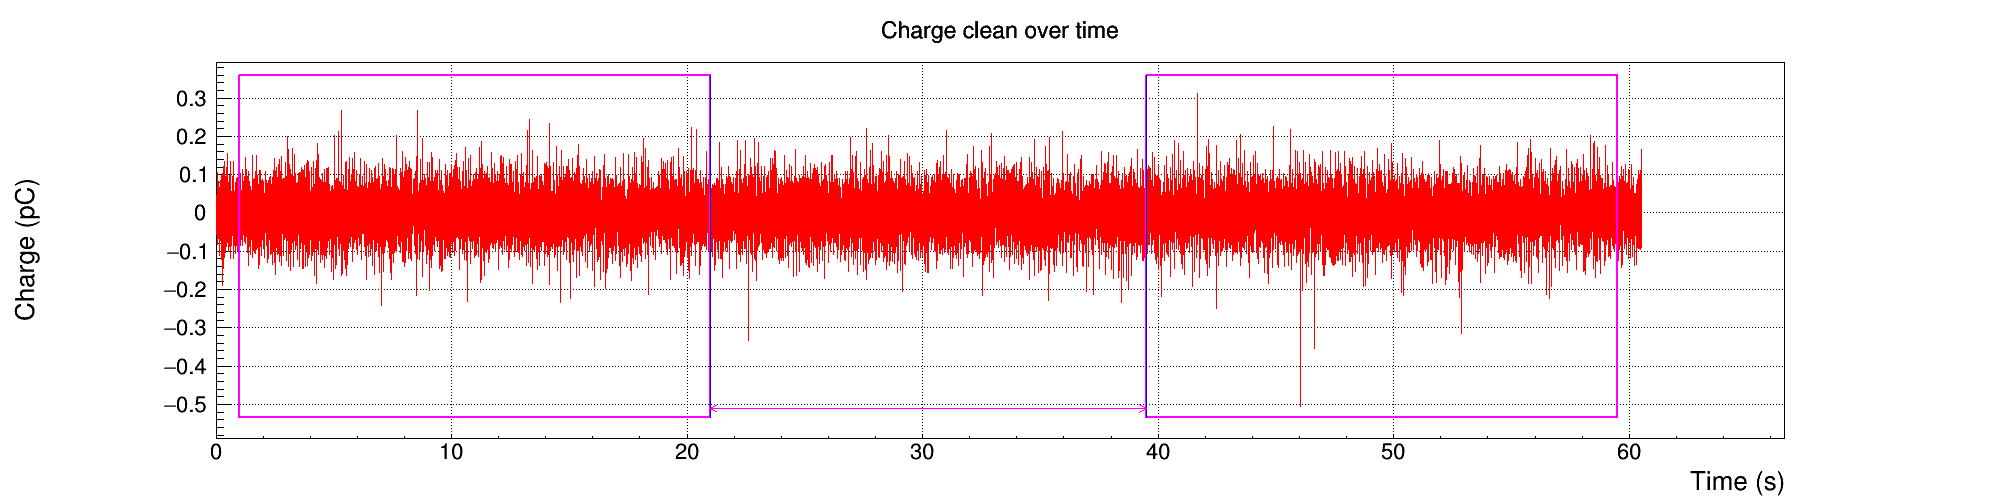
\includegraphics[scale=0.2]{Charge_clean.png} 
\caption{\label{fig:chargec}\footnotesize{Zone d'irradiation « simulée », entre les barres bleues, ainsi que les deux zones, en violet, de bruit l'encadrant}}
\end{center}
\end{figure}
En observant le résultat des soustractions de bruit de fond, et notamment la valeur intégrée de la charge sur la zone fictive du faisceau (la même qu'avec l'actuel faisceau), nous pouvons évaluer la justesse de notre méthode de calcul.
\begin{figure}[h]
\begin{center}
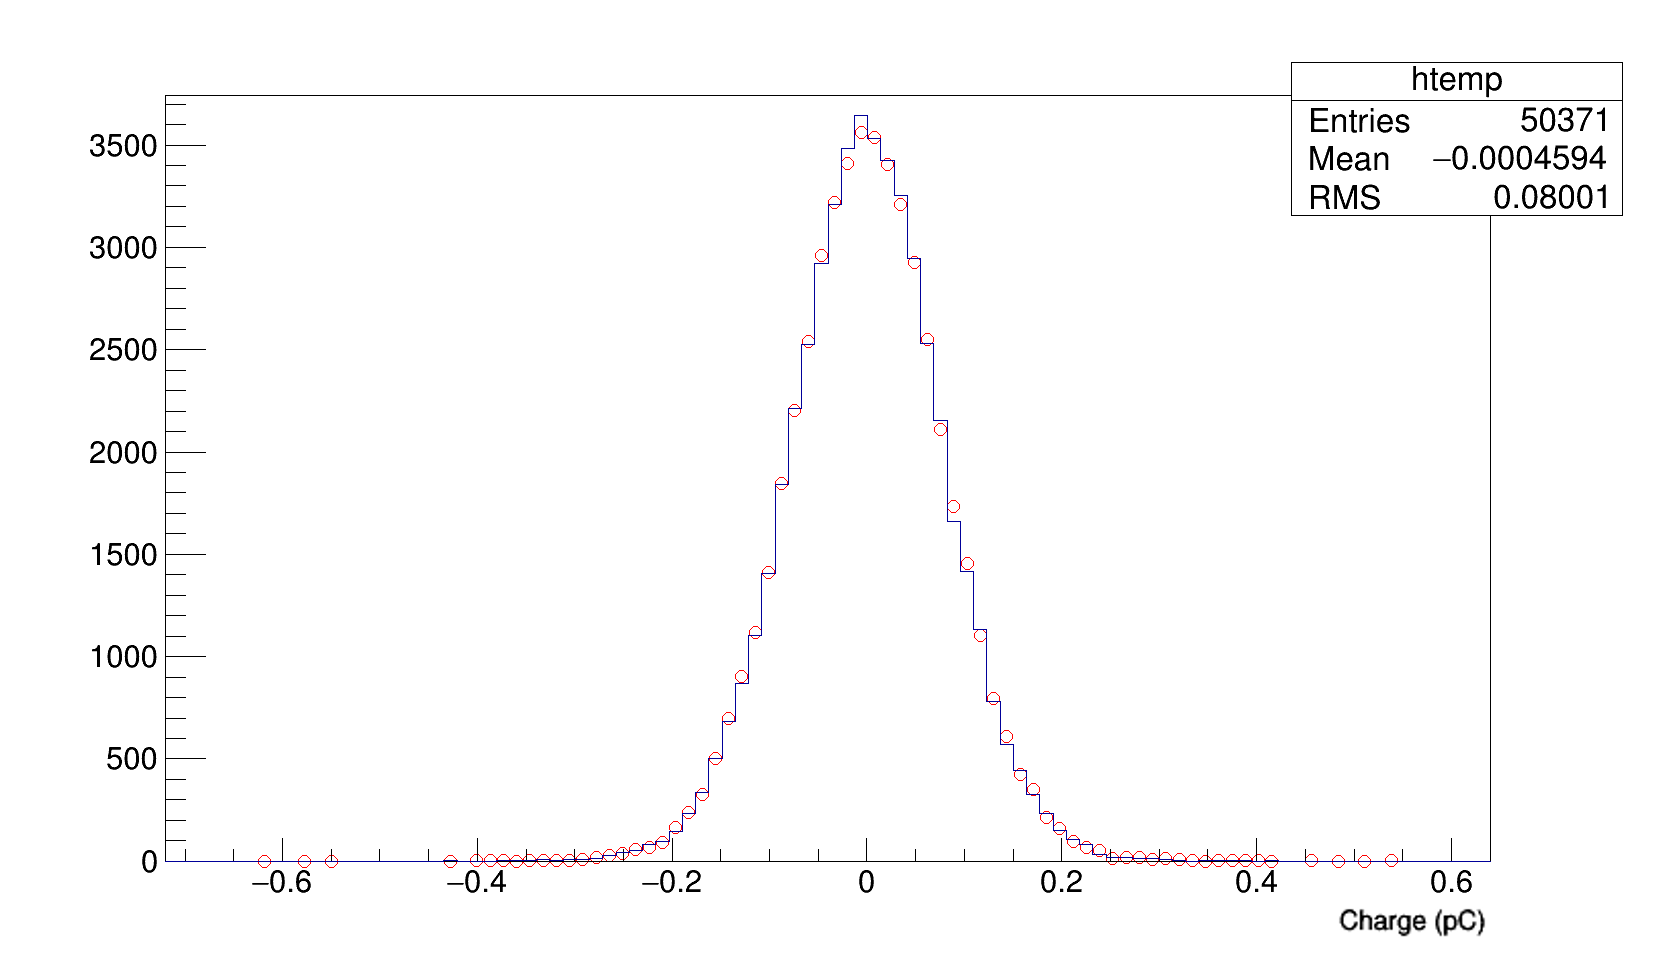
\includegraphics[scale=0.2]{Canvas_1.png} 
\caption{\label{fig:canvas}\footnotesize{Charge intégrée sur toutes les pistes (ligne bleue) et sur les seules pistes irradiées (ronds rouges)}}
\end{center}
\end{figure}
Dans les deux cas les distributions sont parfaitement centrées en 0 et leur déviation standard est de l'ordre de 80 fC.
Cela montre où se situe le niveau de précision que nous pouvons espérer atteindre.

A titre de comparaison, nous avons réalisé la même étude sans utiliser l'ajustement trame par trame mais uniquement une soustraction du bruit électronique. 
Les résultats montrent un décalage du centre, une déformation de la gaussienne ainsi qu'une augmentation de la déviation standard, figure \ref{fig:canvaspp}.
Cela nous conforte d'autant plus quant à la viabilité de cet ajustement trame par trame.
\begin{figure}[h]
\begin{center}
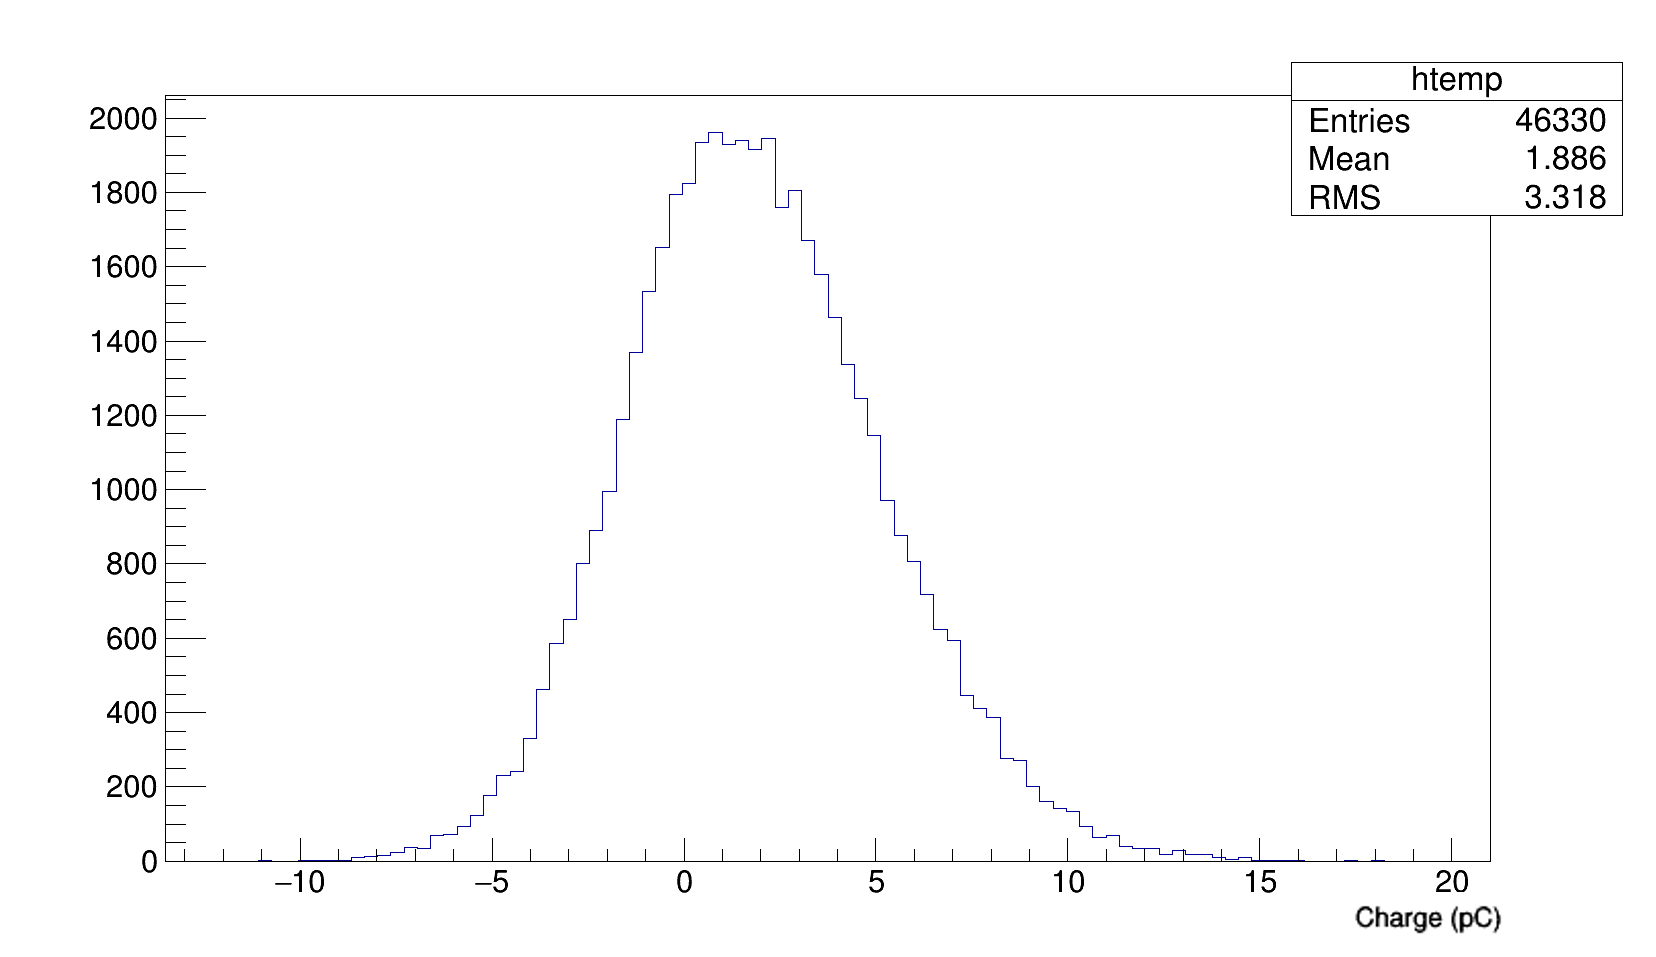
\includegraphics[scale=0.2]{Canvas_1pp.png} 
\caption{\label{fig:canvaspp}\footnotesize{Charge intégrée sur toutes les pistes sans ajustement trame par trame du bruit de fond.}}
\end{center}
\end{figure}

\subsection*{Calibrage de Dosion}
Maintenant que nous sommes capables de soustraire plus efficacement le bruit de fond, nous pouvons analyser les fichiers de calibrage de Dosion.
Nous possédons des mesures pour cinq différents points en énergie, ainsi que cinq mesures différentes pour un même point, celui de plus haute énergie (position 0 de la roue). 
L'analyse de ces neuf fichiers nous amène à la courbe \ref{fig:calibp}.
\begin{figure}[h]
\begin{center}
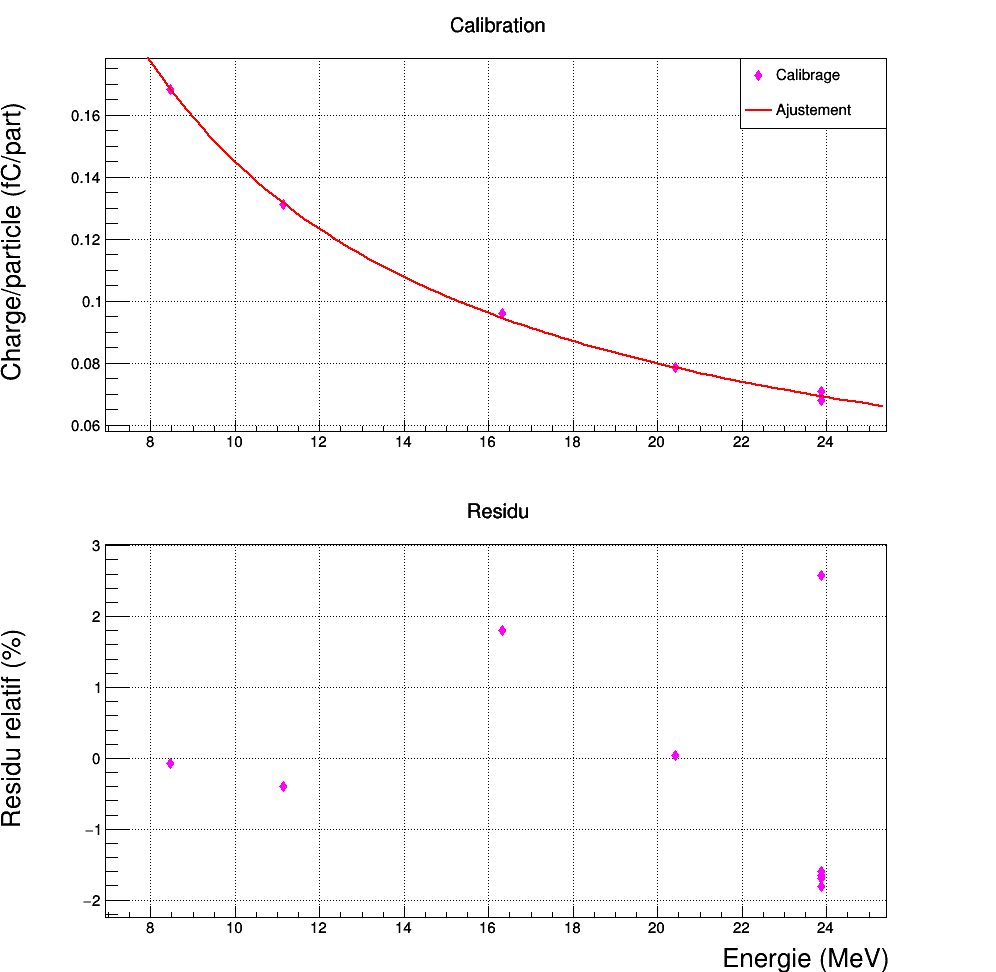
\includegraphics[scale=0.4]{Calibrationp.png} 
\caption{\label{fig:calibp}\footnotesize{Valeurs obtenues pour le calibrage ainsi que la courbe d'ajustement (en haut) et le résidu relatif de chaque valeur (en bas)}}
\end{center}
\end{figure}

Hormis pour le point obtenu sous une irradiation de 2 pA, pour lequel la réponse du PM a peut-être été mal maîtrisée du fait de cette intensité plus élevée, nous notons une très bonne reproductibilité de nos mesures.

Les deux irradiations complètes de la roue réalisées avec le PM et pour lesquelles nous avons sauvegardé les valeurs du scaler vont nous permettre d'obtenir, en analysant chaque période d'irradiation une à une, des valeurs de calibrages pour toute la gamme en énergie. 
Le point de plus basse énergie a dû cependant être exclu, car la réponse du PM n'était plus exploitable.
\begin{figure}[h]
\begin{center}
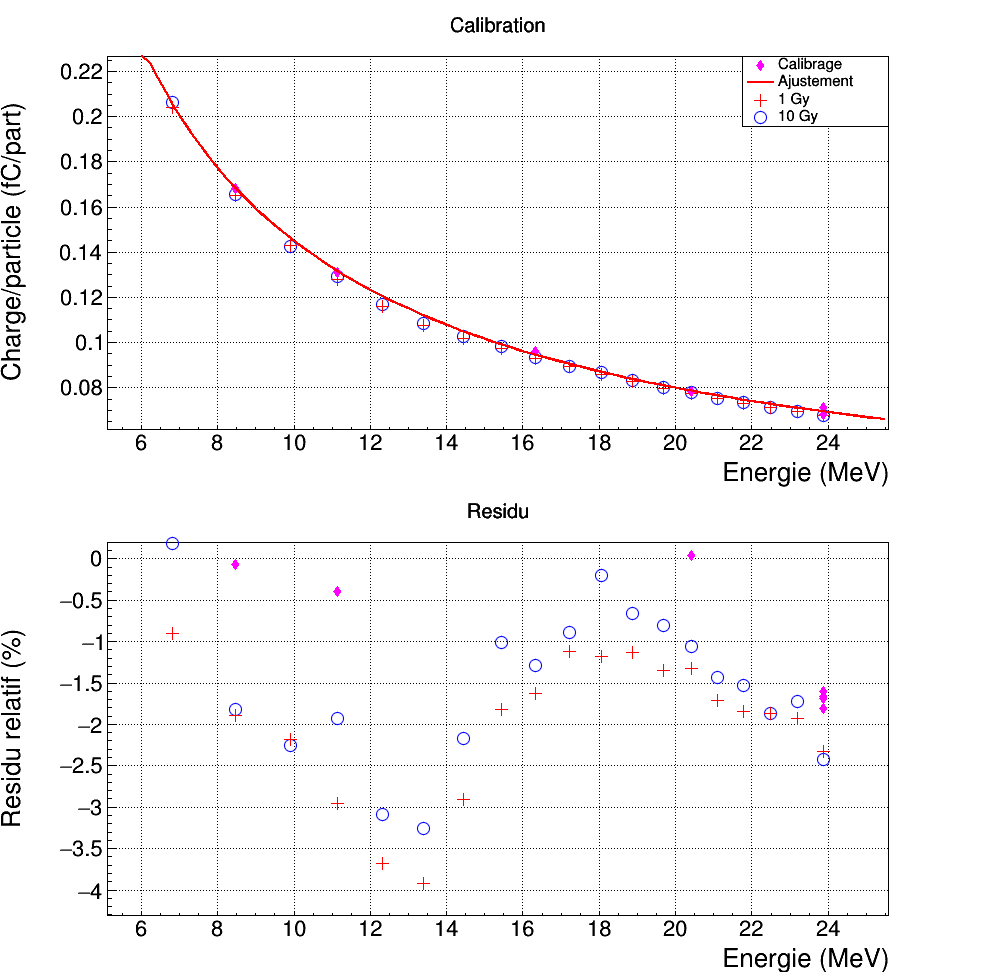
\includegraphics[scale=0.4]{Calibration.png} 
\caption{\label{fig:calib}\footnotesize{Valeurs obtenues pour les irradiations complètes ainsi que leurs résidus relatifs respectifs}}
\end{center}
\end{figure}

Les résultats semblent cohérents entre eux, notamment pour les points obtenus lors des deux séries d'irradiation complète. 
La fonction d'ajustement est du type $f(x)\propto 1/x$ avec $x$ l'énergie des particules, pour correspondre à la loi de Bethe-Bloch.
Nous remarquons que la forme des erreurs est très semblable entre les trois séries de données.
Nous notons également que la valeur de calibrage est très dépendante de l'énergie des particules et que c'est un paramètre qu'il faudra prendre en compte.

\subsection*{Retour sur contrôle commande}
Un des aspects qui vous intéresse sur \cyrce\ quant à l'utilisation du Dosion, est de pouvoir vous en servir comme contrôleur de dose en direct et lui donner la main pour qu'il stoppe l'irradiation une fois la dose prescrite atteinte.
Étant donné les calculs nécessaires, bruit de fond, valeurs de calibrage différentes, il n'est pas possible d'intégrer directement cette méthode de contrôle dans Faster. 
En revanche il est possible de traiter les données en sortie directe de Faster par l'intermédiaire d'un tube nommé. 
Pour résumer, Faster stocke les données en sortie non plus dans un fichier, mais dans un tube qui est lu par un programme lancé en parallèle et se chargeant de faire toute l'analyse, de stocker tout de même les données dans un fichier (permettant un contrôle à posteriori), et d'envoyer le signal lorsque la dose prescrite est atteinte.
J'ai écrit un programme réalisant ces opérations que j'ai testé sur des fichiers Faster rejoués. 
Cela semble fonctionner sans soucis, la soustraction du bruit de fond est bien réalisée en direct, et un signal peut être envoyé une fois la condition de fin atteinte.
Il y a cependant trop d'inconnues, notamment sur la façon avec laquelle le cyclotron est commandé, pour que j'en dise plus quant à la viabilité de cette méthode. 
Toutefois, après en avoir parlé avec les personnes travaillant au développement du code de Faster, c'est peut-être la méthode la plus efficace. 
Certaines précautions sont à prendre, particulièrement veiller à ce que le temps nécessaire aux différents calculs ne soit pas supérieur au temps d'intégration de l'acquisition, dans mes tests il était de 2.4 ms et cela a parfaitement fonctionné.

\subsection*{Analyse fichiers d'irradiation complète}
Lorsque j'ai analysé les derniers fichiers obtenus sans PM, et qui concernent les irradiations de 10 Gy à 10 pA, j'ai pu remarquer un écart entre les deux tirs.
Cet écart étant constant, environ 9\%, sur toute la durée, et les temps de passage pour chaque épaisseur de roue identiques d'une irradiation à l'autre, je pense qu'il provient tout simplement d'une différence d'intensité entre les deux tirs.
Je ne me souviens plus si lors de ces tirs nous avions juste attendu une stabilisation de l'intensité à à peu près 10 pA, mais dans un cas comme celui-là Dosion aurait effectivement pu adapter les différents temps d'irradiation pour que la dose s'ajuste à la prescription.
L'analyse de ces fichiers à également montré que l'écart de charges mesurées entre les chambres X et Y est toujours constant, le rapport des charges X sur Y tourne autour de 97\% (la déviation standard étant inférieure au pourcent sur l'ensemble des mesures).
Cet écart peut s'expliquer tout simplement par le fait que X était placé avant Y, mais également par des épaisseurs de gap différentes.
Un test peut être envisagé où Dosion est placé de telle sorte que la chambre Y est irradiée la première.

\subsection*{Perspectives}
Concernant le bruit de fond particulier observé sur \cyrce , il aurait été intéressant de jouer avec les temps d'intégration. 
En l'augmentant nous aurions pu voir si finalement le bruit se moyenne sur l'ensemble des pistes et ainsi nous affranchi d'une extraction trame par trame. 
Cela pourra notamment se montrer intéressant si le traitement trame par trame prend trop de temps pour une utilisation en direct. 
Diminuer le temps d'intégration nous aurait peut-être permis de mieux identifier l'origine de ce bruit et d'ainsi le réduire à sa source.
J'ajoute cependant que nous avons observé le même phénomène au CPO où les conditions d'irradiations y sont un peu différentes, la Dosion n'étant notamment pas solidaire de la ligne du faisceau ce qui le coupe des vibrations engendrées par les pompes à vides.

Comme dit, l'ajustement utilisé pour la soustraction trame par trame est loin d'être optimal, je l'ai choisi car c'était le plus simple à mettre en place et qu'il m'a permis d'avoir rapidement une réponse quant à la validité d'un tel traitement. 
Par la suite, il faut peut-être envisager une autre méthode, plus rapide et rigoureuse.

Pour le calibrage, il sera peut-être judicieux de procéder à une mesure avec une meilleure statistique aux points de plus basse énergie, je ne suis pas sûr que l'ajustement les « prend bien en compte ».

Pour le retour contrôle commande il y a là beaucoup de questions qui pourront être résolues après des discussions, mais dans la pratique c'est quelque chose de possible et de relativement simple à mettre en place.

\newpage

\begin{center}
\subsection*{Analyse des données issues des irradiations sur \cyrce\ (Mars 2018)}
\end{center}

\subsubsection*{Notes :}
Les valeurs en énergie ont été recalculées par l'IPHC ce qui explique qu'elles soient un peu différentes des précédentes.
L'origine du bruit microphonique a également été trouvée, il s'agit du système de refroidissement de la salle du cycloctron.
Indispensable pour de longues irradiations, il peut toutefois être coupé l'espace de quelques minutes.
Le collimateur utilisé pour l'ensemble des irradiations était de 1.65 mm.

\subsection*{Rappel de l'ensemble des irradiations}
\begin{center}
\begin{tabular}{lrrrrl}
Fichier&pA&pos.&MeV&Gy&Notes\\
\hline
\hline
Dosion\_01\_03\_calib\_01&0.8&0&23.71&&Soucis de multi-irradiations\\
Dosion\_01\_03\_calib\_02&0.6&0&23.71&&\\
Double\_PM\_01&2.0&0&23.71&&Branchement Y du D1 mal effectué\\
Double\_PM\_02&2.0&0&23.71&&\\
Double\_PM\_pt\_01&2.0&pt&&&\\
Double\_PTW\_pos0\_04&1.2&0&23.71&&PTW=155 pC\\
Double\_PTW\_pos2\_02&1.2&2&22.30&&PTW=134 pC\\
Double\_PTW\_pos4\_02&1.2&4&20.90&&PTW=116 pC\\
Double\_PTW\_pos6\_02&1.2&6&19.46&&PTW=99 pC\\
Double\_PTW\_pos8\_02&1.2&8&17.83&&PTW=86 pC\\
speed\_bis&&0&23.71&&Fichier test du contrôle en ligne\\
\hline
\end{tabular}
\end{center}


%%%%%%%%%%%%%%%%%%%%%%%%%%%%%%%%%%

\end{document}

%%%%%%%%%%%%%%%%%%%%%%%%%%%%%%%%%%%%%%%%%%%%%%%%%%%%%%%%%%%%%%%%%%%%%%%%%%%%%%%%%%%%%%%%%%%%%%%%%%